\documentclass{sig-alternate}
%\usepackage{color}
%\usepackage[colorinlistoftodos]{todonotes}
\usepackage{graphicx}
\usepackage{multirow}

%%%%% Uncomment the following line and comment out the previous one
%%%%% to remove all comments
%%%%% NOTE: comments still occupy a line even if invisible;
%%%%% Don't write them as a separate paragraph
%\newcommand{\mycomment}[1]{}

\begin{document}

% --- Author Metadata here ---
%%% REMEMBER TO CHANGE THE SEMESTER AND YEAR
\conferenceinfo{UMM CSci Senior Seminar Conference, April 2014}{Morris, MN}

\title{Morphological Operations Applied to Crack Detection in Digital Art Restoration}

\numberofauthors{1}

\author{
% The command \alignauthor (no curly braces needed) should
% precede each author name, affiliation/snail-mail address and
% e-mail address. Additionally, tag each line of
% affiliation/address with \affaddr, and tag the
% e-mail address with \email.
\alignauthor
M. Kirbie Dramdahl\\
	\affaddr{Division of Science and Mathematics}\\
	\affaddr{University of Minnesota, Morris}\\
	\affaddr{Morris, Minnesota, USA 56267}\\
	\email{dramd002@morris.umn.edu}
}

\maketitle
\begin{abstract}
This paper provides an overview of the processes involved in detecting and removing cracks from digitized works of art. Specific attention is given to the crack detection phase as completed through the use of morphological operations. Mathematical morphology is an area of set theory applicable to image processing, and therefore lends itself effectively to the digital art restoration process.
\end{abstract}

%\category

%\terms

\keywords{mathematical morphology, edge detection, crack detection, crack removal, inpainting, digital art restoration}

\section{Introduction}\label{introduction}
The restoration of paintings and other works of art is an important aspect in preserving objects of artistic, cultural, or historic significance. However, this is also an expensive, demanding, and time-consuming process reserved for the abilities of specialists \cite{Theran:2013}. For this reason, the process of digital art restoration has been developed, which provides both a comparatively inexpensive alternative and a nondestructive tool to be used in the planning of physical restoration. Additionally, digital art restoration allows art historians an approximation of the initial form of a work \cite{TopHat:2010}.

While there are many forms of damage a piece of art may accumulate over time, one of the most common deteriorations is cracking. These cracks, or \textit{craquelure}, may form as a result of climate, drying, or mechanical factors \cite{Altarpiece:2013, Statistics:2013, TopHat:2010}. This paper examines the detection and removal of cracks from pieces of digitized art. The main emphasis is on the detection phase, as carried out by mathematical morphology, which is a method of image processing based in set theory.

This paper breaks the digital art restoration process into three steps: edge detection, crack detection, and crack removal. Section \ref{edge detection} covers edge detection by examining an optimal edge detector known as the Canny edge detection algorithm. Section \ref{morphological operations} provides an examination of the four basic morphological operators of erosion, dilation, opening, and closing. This information is necessary to understanding section \ref{crack detection}, which covers crack detection, and is the main focus of this paper. Section \ref{inpainting} wraps up the digital art restoration process in covering the crack removal process (known as \textit{inpainting}). The remaining sections provide a summary. Section \ref{results} reviews the results obtained by various methods of digital art restoration, again with a specific focus on the success of various morphological operators in the crack detection stage, and section \ref{conclusion} provides a summary of the information provided in this paper, as well as discusses possible further areas of interest and study.

\section{Edge Detection}\label{edge detection}
Edges within a digitalized work of art are boundaries between areas of varying intensity. In other words, an edge occurs where there is ``a jump in intensity from one pixel to the next'' \cite{CannySummarized}. Intensity, in art, is defined as brightness or dullness of a color; the brighter the color, the higher its intensity. For example, in greyscale images, white has the highest intensity and black has the lowest intensity.

Edge detection is actually not necessary to the crack detection and removal process, and does not rely on mathematical morphology. However, this paper provides a brief discussion of the process for two reasons. The first is that edge detection provides the advantage of reducing the amount of data to be processed while still preserving the necessary edge information. The second is that the choice of whether or not edge detection is used affects the morphological filters used later in the crack detection and removal process \cite{CannySummarized}. While there are several possible methods of edge detection, this paper will examine the Canny algorithm \cite{Canny:1986, CannySummarized}.

The Canny algorithm is based upon three criteria, which are as follows \cite{Canny:1986, CannySummarized}:
\begin{enumerate}
\item Accuracy - The edge detection algorithm should have a low error rate. This implies that there should be neither false positives (edges detected where they do not exist) nor false negatives (edges not detected where they do exist).
\item Localization - The edge detection algorithm should minimize the distance between the edge detected and the actual edge.
\item Uniqueness - The edge detection algorithm should have only one response to a single edge.
\end{enumerate}

In order to fulfill these criteria, the Canny algorithm first uses a Gaussian filter to smooth the image. Having eliminated noise, the algorithm then takes the gradient of the image. An image gradient is a map of the directional changes in intensity within an image. The gradient is then used to locate regions where there are significant jumps in intensity. The regions identified here are then searched for local maximum. All non maximum pixels are set to zero. In the final step, the Canny algorithm further refines the detected edges by comparing the remaining pixels to two thresholds. If the intensity of a pixel falls below the low threshold, it is set to zero. If the intensity of a pixel falls above the high threshold, it is set to one (made an edge). If the intensity of a pixel falls between the two thresholds, it is set to one if at least one adjacent pixel has an intensity above the high threshold, and set to zero otherwise \cite{CannySummarized}. The result of the Canny algorithm is a binary image depicting the edges of the initial input image.

\section{Morphological Operations}\label{morphological operations}
Following optional edge detection is crack detection, the focus of this paper. However, in order to understand this stage, it is first necessary to describe the basic principles of mathematical morphology. Typically, morphology is used in processing binary (black and white) images, although there are also variations used for greyscale images. This paper will examine both variations. Morphological functions take two inputs. The first input is the image to be processed. In binary morphology, the input image is divided into foreground (typically white) and background (typically black) regions. In greyscale morphology, the image is treated as a three-dimensional surface, where higher areas are brighter (white) and lower areas are darker (black). The second input is a structuring element, a (typically small, in comparison to the image) set of coordinate points. An example of a 3x3 square structuring element with the origin located at the center in comparison to both a 30x20 binary image and an 11x32 greyscale image is presented in Figure \ref{structuring element figure}. The structuring element is then used to modify the input image. The image that results from the morphological operation is determined by the shape, size, and point of origin of the structuring element \cite{MorphologyWikiAnonymous, MorphologyBook:2000, MorphologyPaper:1987, MorphologyWiki}. Subsections \ref{erosion}, \ref{dilation}, \ref{opening}, and \ref{closing} explain the fundamental operations of mathematical morphology.
\begin{figure}
\centering
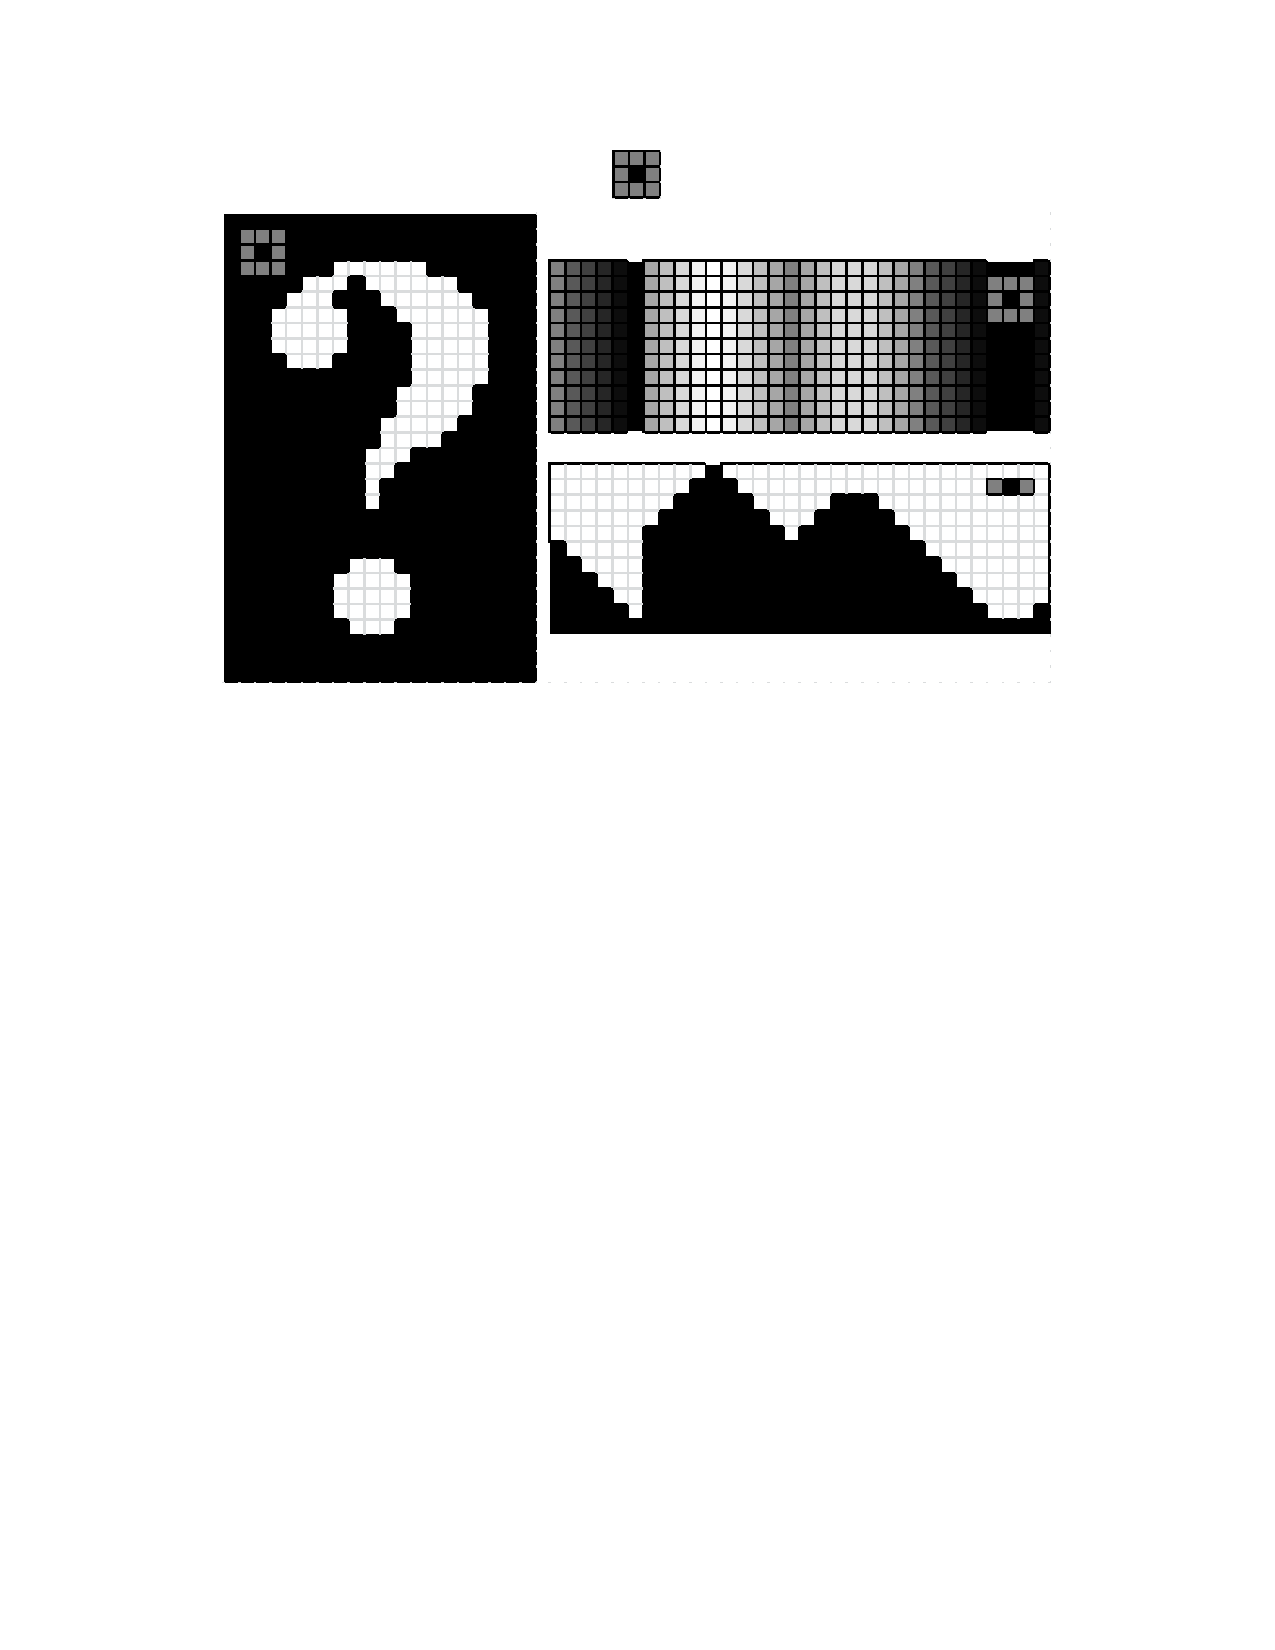
\includegraphics[width=3in,trim={0 6.5in 0 0},clip]{structuring_element}
\caption{Structuring Elements: Top: Structuring Element. Bottom Left: Structuring Element in Comparison to Binary Image. Bottom Right: Structuring Element in Comparison to Greyscale Image (Above) and Cross-Section (Below).}
\label{structuring element figure}
\end{figure}

\subsection{Erosion}\label{erosion}
Erosion of an image strips away a layer of pixels from the boundaries of foreground regions, and is denoted by the equation
\begin{equation*}
g = f \ominus s
\end{equation*}
where \textit{g} is the resulting image, \textit{f} is the original image, and \textit{s} is the structuring element. The symbol $\ominus$ indicates erosion \cite{MorphologyWikiAnonymous, MorphologyBook:2000}.

In binary erosion, erosion is accomplished by placing the origin of the structuring element over every pixel of the foreground regions in turn. If every point within the structuring element is in line with a foreground pixel, the foreground pixel lined up with the origin of the structuring element is left unchanged. If at least one point within the structuring element is in line with a background pixel, then the pixel lined up with the origin of the structuring element is converted to a background pixel \cite{MorphologyWiki}. An example of binary erosion on a 30x20 image using a 3x3 square structuring element with the origin located at the center is presented in Figure \ref{binary erosion figure}. The erosion of foreground regions is equivalent to the dilation (discussed in subsection \ref{dilation}) of background regions \cite{MorphologyWiki}.
\begin{figure}
\centering
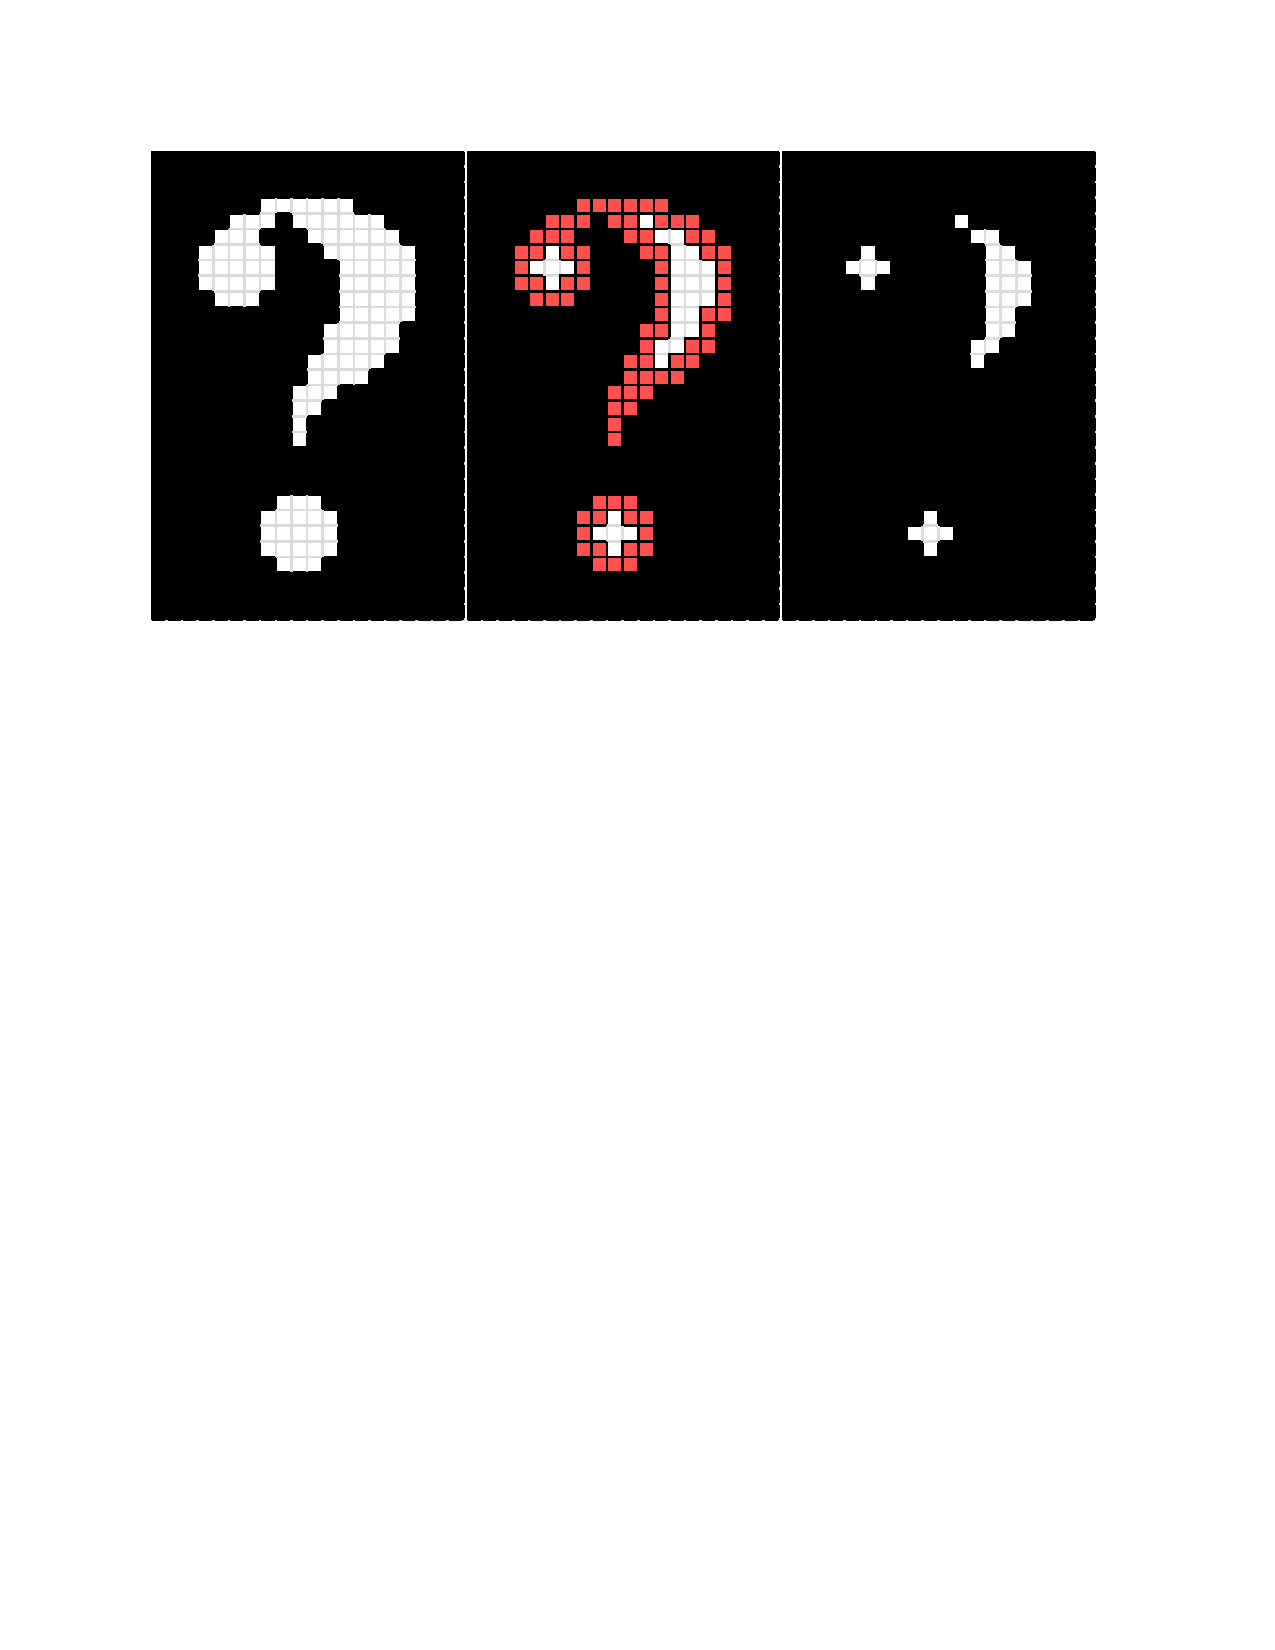
\includegraphics[width=3in,trim={0 6.75in 0 0},clip]{erosion}
\caption{Binary Erosion: Left: Original Image. Center: Erosion Marked. Right: Results of Erosion.}
\label{binary erosion figure}
\end{figure}

Gray scale erosion follows the same basic pattern, but is somewhat more complex. Here, the origin of the structuring element is placed in line with a pixel on or below the surface. If every point within the structuring element is also either on or below the surface, the pixel lined up with the origin is left unchanged. If at least one point within the structuring element is above the surface, the pixel lined up with the origin of the structuring element is essentially removed (set to be above the surface). This process is repeated for every pixel on or below the surface \cite{MorphologyPaper:1987, MorphologyWiki}. An example of greyscale erosion performed on a cross-section of an 11x32 image using a 3x3 square structuring element with the origin located at the center is presented in Figure \ref{greyscale erosion figure}.
\begin{figure}
\centering
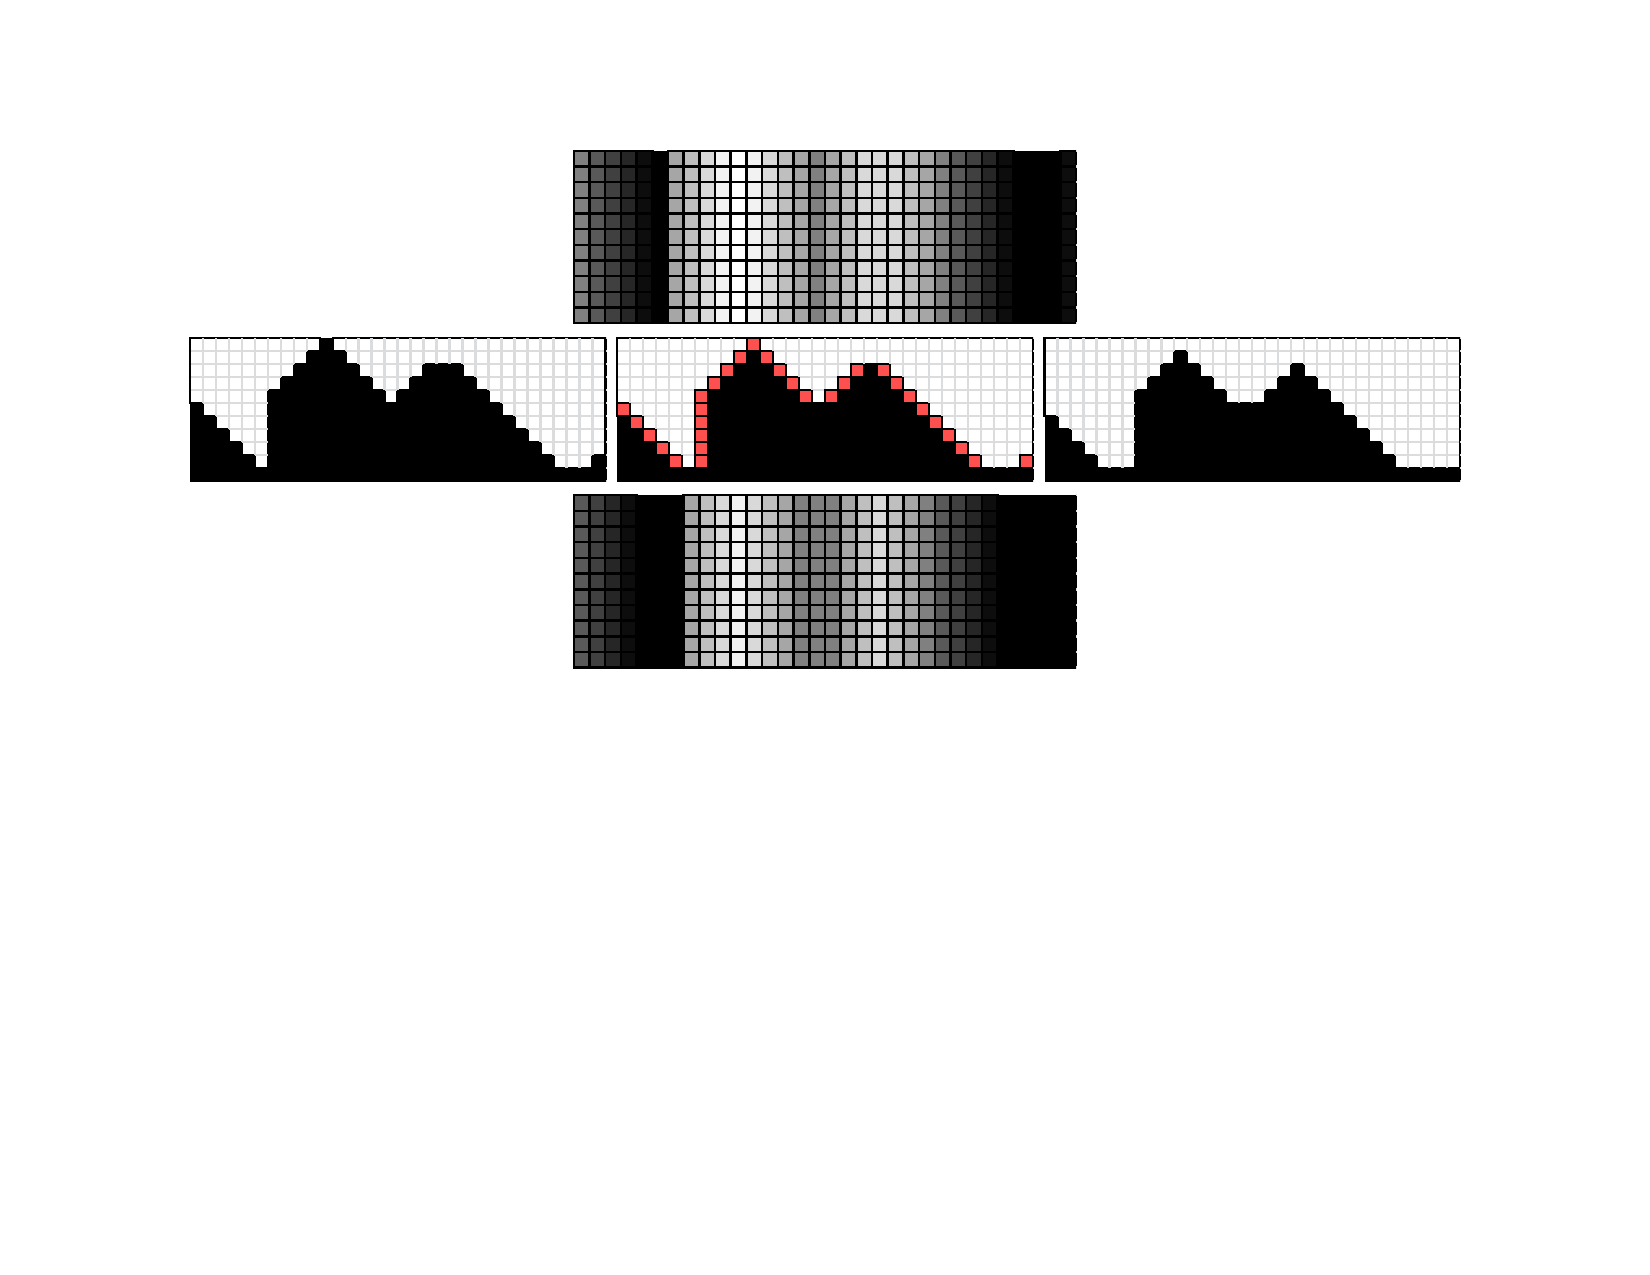
\includegraphics[width=3in,trim={0 4in 0 0},clip]{greyscale_erosion}
\caption{Greyscale Erosion: Top: Original Image. Center Left: Cross-Section of Image Surface. Center Center: Erosion Marked. Center Right: Erosion of Surface. Bottom: Results of Erosion.}
\label{greyscale erosion figure}
\end{figure}

\subsection{Dilation}\label{dilation}
Dilation of an image adds a layer of pixels to the boundaries of foreground regions, and is denoted by the equation
\begin{equation*}
g = f \oplus s
\end{equation*}
where the symbol $\oplus$ indicates dilation \cite{MorphologyWikiAnonymous, MorphologyBook:2000}.

In binary dilation, this is accomplished by placing the origin of the structuring element over every pixel of the background regions in turn. If every point within the structuring element is in line with a background pixel, the background pixel lined up with the origin of the structuring element is left unchanged. If at least one point within the structuring element is in line with a foreground pixel, then the pixel lined up with the origin of the structuring element is converted to a foreground pixel \cite{MorphologyWiki}. An example of binary dilation on a 30x20 image using a 3x3 square structuring element with the origin located at the center is presented in Figure \ref{binary dilation figure}. The dilation of foreground regions is equivalent to the erosion (discussed in subsection \ref{erosion}) of background regions \cite{MorphologyWiki}.
\begin{figure}
\centering

\includegraphics[width=3in,trim={0 6.75in 0 0},clip]{dilation}
\caption{Binary Dilation: Left: Original Image. Center: Dilation Marked. Right: Results of Dilation.}
\label{binary dilation figure}
\end{figure}

Like greyscale erosion, greyscale dilation is a more complex variation its binary counterpart. Here, the origin of the structuring element is placed in line with a pixel above the surface. If every point within the structuring element is also above the surface, the pixel lined up with the origin is left unchanged. If at least one point within the structuring element is on or below the surface, the pixel lined up with the origin of the structuring element is set to be on or below the surface. This process is repeated for every pixel above the surface \cite{MorphologyPaper:1987, MorphologyWiki}. An example of greyscale dilation performed on a cross-section of an 11x32 image using a 3x3 square structuring element with the origin located at the center is presented in Figure \ref{greyscale dilation figure}.
\begin{figure}
\centering
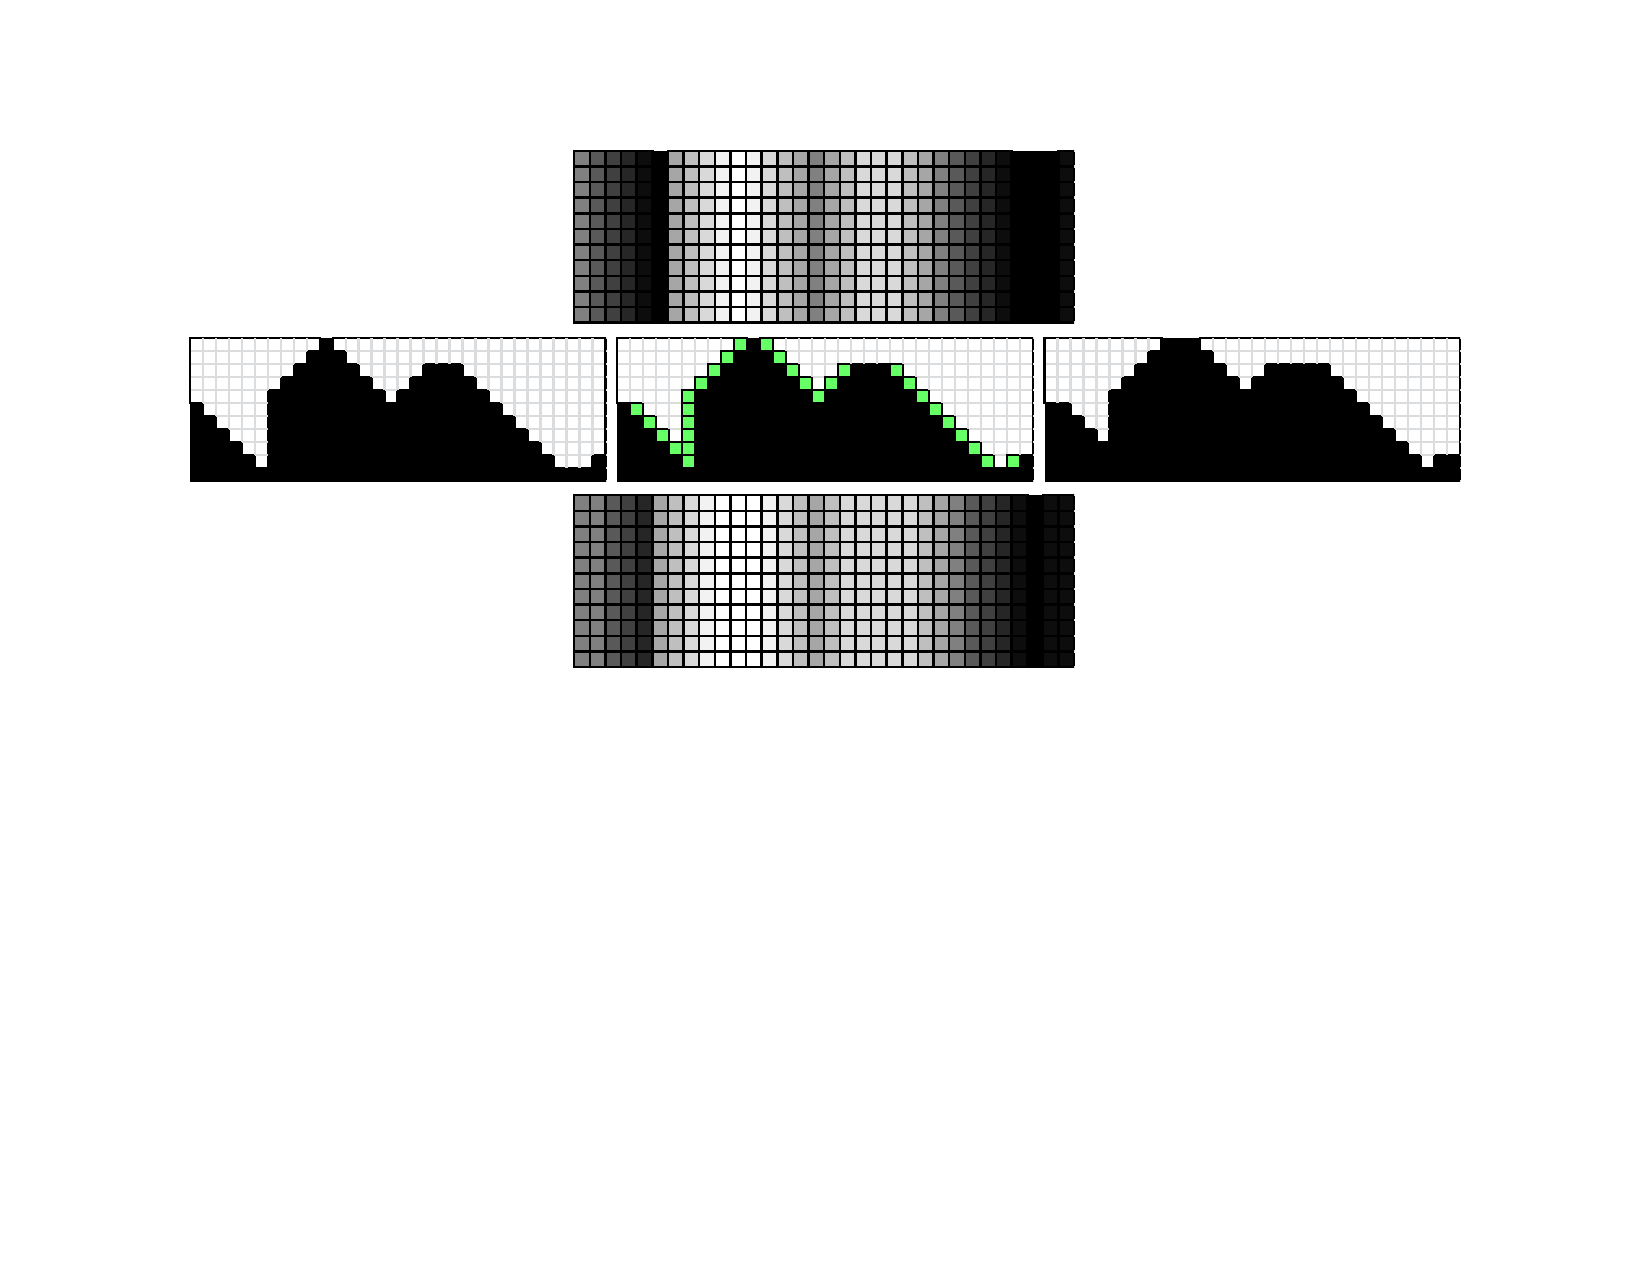
\includegraphics[width=3in,trim={0 4in 0 0},clip]{greyscale_dilation}
\caption{Greyscale Dilation: Top: Original Image. Center Left: Cross-Section of Image Surface. Center Center: Dilation Marked. Center Right: Dilation of Surface. Bottom: Results of Dilation.}
\label{greyscale dilation figure}
\end{figure}

\subsection{Opening}\label{opening}
The opening of an image is an erosion followed by a dilation, and is denoted by the equation
\begin{equation*}
g = f \circ s = (f \ominus s) \oplus s
\end{equation*}
where the symbol $\circ$ indicates opening \cite{MorphologyWikiAnonymous, MorphologyBook:2000}. Similar to erosion, opening strips away foreground pixels at the boundaries of foreground regions, but is less destructive of the initial foreground regions than erosion. Opening is therefore typically used to preserve foreground regions with a similar size and shape to the structuring element, while removing or reducing other foreground regions \cite{MorphologyWiki}. An example of binary opening on a 30x20 image using a 3x3 square structuring element with the origin located at the center is presented in Figure \ref{binary opening figure}. The opening of foreground regions is equivalent to the closing of background regions \cite{MorphologyWiki}.
\begin{figure}
\centering
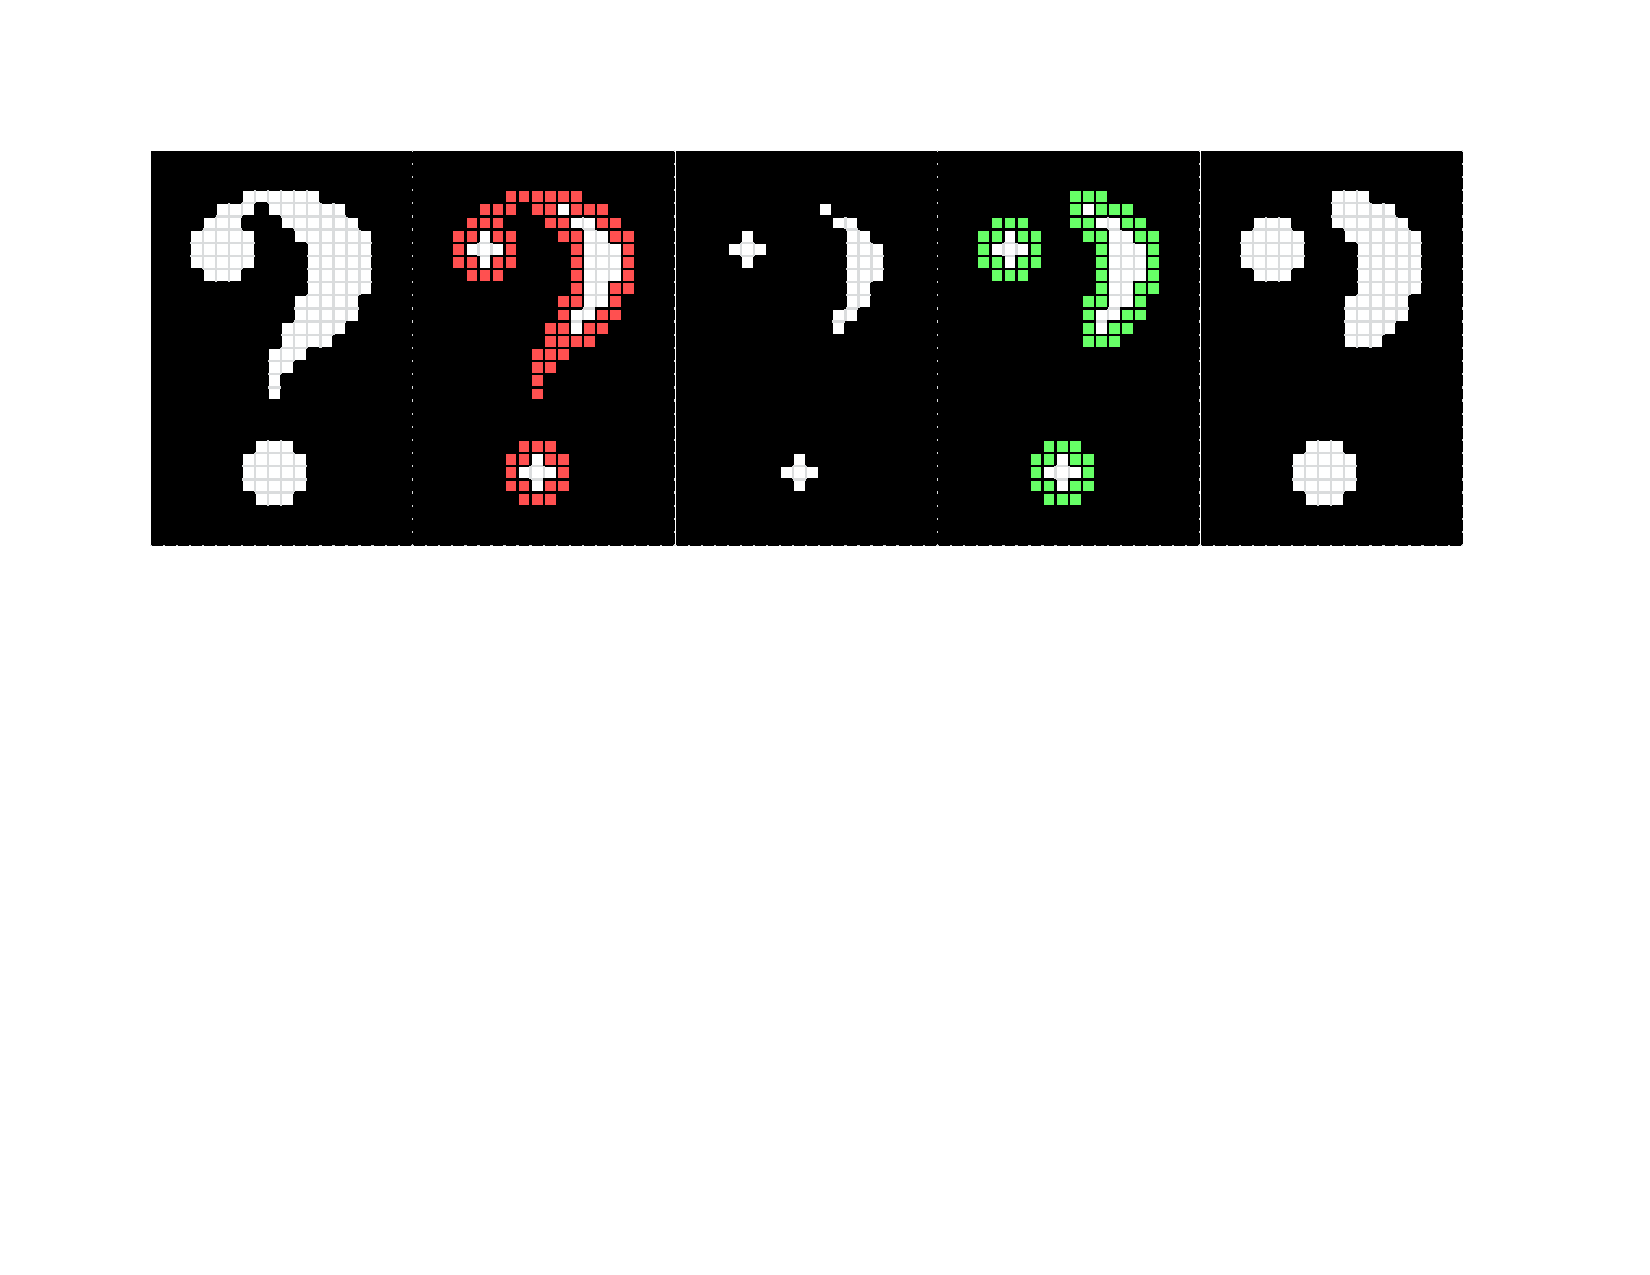
\includegraphics[width=3in,trim={0 4.75in 0 0},clip]{opening}
\caption{Opening: Left: Original Image. Second from Left: Erosion Marked. Center: Results of Erosion. Second from Right: Dilation Marked. Right: Results of Dilation (Opening Complete).}
\label{binary opening figure}
\end{figure}

The greyscale opening of an image also consists of an erosion followed by a dilation. In this situation, however, both the erosion and dilation are greyscale rather than binary \cite{MorphologyPaper:1987}.

\subsection{Closing}\label{closing}
Closing of an image is a dilation followed by an erosion, and is denoted by the equation
\begin{equation*}
g = f \bullet s = (f \oplus s) \ominus s
\end{equation*}
where the symbol $\bullet$ indicates closing \cite{MorphologyWikiAnonymous, MorphologyBook:2000}. Similar to dilation, closing adds foreground pixels at the boundaries of foreground regions, but is less destructive of the initial background regions than dilation. Closing is therefore typically used to preserve background regions with a similar size and shape to the structuring element, while removing or reducing other background regions \cite{MorphologyWiki}. An example of binary closing on a 30x20 image using a 3x3 square structuring element with the origin located at the center is presented in Figure \ref{binary closing figure}. The closing of foreground regions is equivalent to the opening of background regions \cite{MorphologyWiki}.
\begin{figure}
\centering

\includegraphics[width=3in,trim={0 4.75in 0 0},clip]{closing}
\caption{Closing: Left: Original Image. Second from Left: Dilation Marked. Center: Results of Dilation. Second from Right: Erosion Marked. Right: Results of Erosion (Closing Complete).}
\label{binary closing figure}
\end{figure}

The greyscale closing of an image also consists of a dilation followed by an erosion. In this situation, however, both the dilation and erosion are greyscale rather than binary \cite{MorphologyPaper:1987}.

\section{Methods of Crack Detection}\label{crack detection}
The next step in the crack detection and removal process (following optional edge detection), is crack detection. This section will discuss the application of various morphological filters to this problem.

\subsection{Top-Hat Transform}
The morphological filter most frequently used for detecting cracks within digitalized works of art is the top-hat transform. There are two variations on this filter, the black top-hat transform and white top-hat transform, which will be discussed in subsubsections \ref{black top-hat} and \ref{white top-hat} respectively.

\subsubsection{Black Top-Hat}\label{black top-hat}
The black top-hat transform (also referred to as the closing top-hat transform) is used for detecting darker details on a lighter background within greyscale images\cite{Altarpiece:2013, TopHat:2010}. This transform is defined as the difference between the closing of the original image by a specified structuring element and the original image itself, and is denoted by the equation
\begin{equation*}
BTH = (f \bullet s) - f
\end{equation*}
where \textit{f} is the original image and \textit{s} is the structuring element. This transformation produces a greyscale image with the desired details enhanced.

\subsubsection{White Top-Hat}\label{white top-hat}
The white top-hat transform (also referred to as the opening top-hat transform or, sometimes, the bottom-hat transform), is used for detecting lighter details on a darker background within greyscale images\cite{Altarpiece:2013, TopHat:2010}. This transform is defined as the difference between the original image itself and the opening of the original image by a specified structuring element, and is denoted by the equation
\begin{equation*}
WTH = f - (f \circ s)
\end{equation*}
where \textit{f} is the original image and \textit{s} is the structuring element. Like its counterpart, this transformation produces a greyscale image with the desired details enhanced.

\subsubsection{Multiscale Top-Hat}\label{multiscale top-hat}
Subsubsections \ref{black top-hat} and \ref{white top-hat} explain classical top-hat transforms. While these are popular and frequently used, they are not perfect. Paintings often contain details (such as fine brush strokes) which are misinterpreted as cracks by these filters. The multiscale morphological top-hat transform may be used to counteract this, as well as to detect cracks of varying sizes \cite{Altarpiece:2013}. This transformation is executed by performing a series of classical top-hat transforms with structuring elements of various shapes and sizes (Cornelis et al use square structuring elements "ranging from 3x3 to \textit{n}x\textit{n} pixels, where \textit{n} depends on the width of the crack to be detected" \cite{Altarpiece:2013}). The resulting images, or crack maps, are then further processed to remove isolated groups of pixels and bridge pixel gaps.

At this point, the crack maps are combined in order to build one final, comprehensive crack map. Cornelis et al accomplish this by first combining the crack maps derived from the three smallest structuring elements (the finer, thinner cracks) in what is referred to as the base map \cite{Altarpiece:2013}. From here, the crack maps derived from the larger structuring elements (the coarser, heavier cracks) are layered onto the base map. This is done by only adding those coarser cracks which are connected to the finer cracks of the base map. The resulting final crack map both contains cracks of a variety of scales and reduces the occurrence of false positives \cite{Altarpiece:2013}.

\subsection{Alternative Methods}\label{alternative}
While the top-hat method is the most common morphological filter applied to the problem of crack detection in digital art restoration, there are other methods of finding a solution. Karianakis and Maragos present one such alternative in their digital restoration of prehistoric Theran wall paintings \cite{Theran:2013}.

In the method implemented by Karianakis and Maragos, the process begins by setting a threshold. If the variation in the intensity of one pixel from its neighbors exceeds the threshold, it is determined to be part of a crack. All other pixels are considered genuine. At this point, morphological closing is applied to the binary image obtained from the previous step. This groups isolated crack pixels, and removes some of the discoloration that may be found around the edges of cracks (this may be a result of light reflecting off paint ridges, or accidental removal of paint during any previous cleaning process \cite{Altarpiece:2013}). The result is the binary mask of cracks \cite{Theran:2013}.

Karianakis and Maragos then return again to the original input image. From this image, the Canny edge detection algorithm (described in section \ref{edge detection}) is used to obtain a binary mask of all edge pixels (both cracks and actual edges within the original painting). Morphological dilation is then applied to the crack mask in order to group any isolated pixels \cite{Theran:2013}.

At this point, Karianakis and Maragos now have two binary masks: the crack mask obtained by thresholding, and the edge map obtained by the Canny edge detection algorithm. These two masks are then joined, and the resulting binary mask is then iteratively eroded until immediately before a certain percentage of edge information is lost. This process results in a smoother crack mask and, depending on how much edge information is lost, reduces the likelihood of false positives \cite{Theran:2013}.

\section{Inpainting}\label{inpainting}
The final stage in the digital art restoration process is crack removal, frequently referred to as inpainting. As with crack detection, there are many potential solutions to the crack removal process. This section will examine the method described by Spagnolo and Somma in their study \cite{TopHat:2010}.

In this method, the original input image is broken down into regions, which are further divided into neighborhoods (Spagnolo and Somma define 5x5 pixel neighborhoods and 100x100 pixel regions \cite{TopHat:2010}). From the previous crack detection step, the defective pixels are already known. For this information, it is now possible to proceed with the inpainting process \cite{TopHat:2010}.

The first step is to select a defective pixel \textit{i}, and to determine its context. The context of a defective pixel \textit{i} consists of all the non-defective pixels in the neighborhood of \textit{i}. From here, all other neighborhoods in the region containing \textit{i} (neighborhoods containing defective pixels are excluded) are examined in order to determine which neighborhood in the region is most similar to the context of the defective pixel \textit{i}. This is done by computing the sum of squared differences between the context of \textit{i} and the corresponding pixels in the neighborhoods within the region of \textit{i}. The neighborhood with the lowest sum of squared differences is determined to be most similar to the context of \textit{i} \cite{TopHat:2010}.

If the sum of squared differences for this similar neighborhood is below a set threshold (that is, if the neighborhood it determined not only to be the most similar to the context of \textit{i}, but also similar enough to be an acceptable match), the defective pixels within the neighborhood of \textit{i} (including \textit{i} itself) are replaced by the corresponding pixels from the ``matched'' neighborhood. If the sum of squared differences is above the threshold, \textit{i} is replaced with the median value of the non-defective pixels within its neighborhood. This process is repeated for every defective pixel \cite{TopHat:2010}.

\section{Results}\label{results}
The final result of the crack detection and removal process depends significantly on the effectiveness of the crack detection method implemented. The results of crack detection may be broken down into four categories, which are as follows \cite{Statistics:2013}:
\begin{itemize}
\item True Positives - Cracks detected where they do exist.
\item False Positives - Cracks detected where they do not exist.
\item True Negatives - Cracks not detected where they do not exist.
\item False Negatives - Cracks not detected where they do exist.
\end{itemize}

One way of evaluating the effectiveness of a particular crack detection algorithm is to determine the occurrences of these various results. Effective algorithms will produce both high rates of true positives and true negatives and low rates of false positives and false negatives, while less effective algorithms will produce low rates of true positives and true negatives, high rates of false positives and false negatives, or a combination of both. There are two methods of simplifying this process. The first is to use these categories to determine false positive rate and true positive rate, respectively denoted by the following equations \cite{Statistics:2013}:
\begin{equation*}
FP = fp / (fp + tn)
\end{equation*}
\begin{equation*}
TP = tp / (tp + fn)
\end{equation*}
where \textit{tp} is the number of true positives, \textit{fp} the number of false positives, \textit{tn} the number of true negatives, and \textit{fn} the number of false negatives. The section option is determine precision (fraction of retrieved instances that are relevant) and recall (fraction of relevant instances that are retrieved), respectively denoted by the following equations \cite{Theran:2013}:
\begin{equation*}
P = tp / (tp + fp)
\end{equation*}
\begin{equation*}
R = tp / (tp + fn)
\end{equation*}
Note that recall is identical to the true positive rate. Subsections \ref{top-hat results} and \ref{alternative results} will examine the effectiveness of the various methods of crack detection discussed in section \ref{crack detection}.

\subsection{Top-Hat Transform Results}\label{top-hat results}
The black top-hat transform and white-transform, discussed in sections \ref{black top-hat} and \ref{white top-hat} respectively, were implemented in the methodology of Desai et al \cite{Statistics:2013}. Prior to crack detection, Desai et al first classified images into three categories: crack thickness, number of cracks, and crack connectivity. In their study, they report both a maximum true positive rate of 0.98 and minimum false positive rate of 0.02 for those images classified by number of cracks. The maximum true positive occurred for images with a moderate number of cracks, while the minimum false positive was obtained from images determined to contain a low number of cracks. On the opposite end of the spectrum, crack connectivity produced both a minimum true positive rate of 0.86 and a maximum false positive rate of 0.124. Both occurred for images with less crack connectivity \cite{Statistics:2013}.

Cornelis et al also made use of the black and white top-hat transforms in their methodology \cite{Altarpiece:2013}. However, while Desai et al used the classical implementation of these algorithms, Cornelis et al instead used the more involved multiscale variation described in subsubsection \ref{multiscale top-hat} \cite{Altarpiece:2013, Statistics:2013}. While Cornelis et al do not provide any statistical data on the success of their algorithm, they do claim that in their restoration of the digitized \textit{Ghent Altarpiece}, the multiscale top-hat transform successfully omitted painting details (such as letters in a book) from the final crack map. These details would otherwise have been determined to be cracks by the classical implementation of the black and white top-hat transforms \cite{Altarpiece:2013}.

\subsection{Alternative Method Results}\label{alternative results}
In comparison, the alternative methodology implemented by Karianakis and Maragos produced significantly different results \cite{Theran:2013}. As previously discussed in subsection \ref{alternative}, the combined edge and crack masks were eroded until a certain amount of edge information was lost. The efficiency of the method relied heavily on the amount of information loss that was permitted. In the case that only 1\% of edge information was discarded, the algorithm resulted in a recall of about 0.932, but a precision of only 0.497. As more edge information is lost, the recall decreases while the precision increases. For example, when 70\% of the edge information is lost, the algorithm reported a recall of only 0.53, but an improved precision of 0.704 \cite{Theran:2013}.

It is evident from the statistics reported (summarized in Table \ref{results table}) that the top-hat transform, in both its classical and multiscale forms, significantly outperforms the alternative implemented by Karianakis and Maragos.
\begin{table}
\centering

\resizebox{8.5cm}{!}{
\begin{tabular}{|l|l|r|r|r|r|r|r|r|}
\hline
\textbf{Method} & \textbf{Classification} & \textbf{\textit{tp}} & \textbf{\textit{fn}} & \textbf{\textit{tn}} & \textbf{\textit{fp}} & \textbf{\textit{TP} (or \textit{R})} & \textbf{\textit{FP}} & \textbf{\textit{P}}\\ \hline
\multirow{8}{*}{Top-Hat Transform}
& Crack Thickness - Thin & 220 & 30 & 230 & 20 & 0.880 & 0.080 & -\\ \cline{2-9}
& Crack Thickness - Medium & 232 & 18 & 231 & 19 & 0.928 & 0.076 & -\\ \cline{2-9}
& Crack Thickness - Thick & 235 & 15 & 238 & 12 & 0.940 & 0.048 & -\\ \cline{2-9}
& Number of Cracks - Few & 242 & 8 & 245 & 5 & 0.968 & \textbf{0.020} & -\\ \cline{2-9}
& Number of Cracks - Medium & 245 & 5 & 241 & 9 & \textbf{0.980} & 0.036 & -\\ \cline{2-9}
& Number of Cracks - Many & 243 & 7 & 243 & 7 & 0.972 & 0.028 & -\\ \cline{2-9}
& Crack Connectivity - Low & 215 & 35 & 219 & 31 & \textbf{0.860} & \textbf{0.124} & -\\ \cline{2-9}
& Crack Connectivity - High & 218 & 32 & 221 & 29 & 0.872 & 0.116 & -\\ \hline
\multirow{3}{*}{Alternative Method}
& Edge Information Lost - 1\% & - & - & - & - & \textbf{0.932} & - & \textbf{0.497}\\ \cline{2-9}
& Edge Information Lost - 30\% & - & - & - & - & 0.857 & - & 0.594\\ \cline{2-9}
& Edge Information Lost - 70\% & - & - & - & - & \textbf{0.530} & - & \textbf{0.704}\\ \hline
\end{tabular}
}
\caption{Crack Detection Results by Methodology: Results Specified in Text Emphasized, Modified from \cite{Statistics:2013, Theran:2013}}.
\label{results table}
\end{table}

\section{Conclusions}\label{conclusion}
This paper has examined digital art restoration by breaking this process down into three primary components: edge detection, crack detection, and crack removal (inpainting), with a specific focus on the crack detection phase as completed using morphological operations.

While it has been demonstrated that there are many and varied effective methods of crack detection and removal, cracks are only one form of defect that may be encountered in the digital art restoration process. Areas for further study include the detection and removal of dust, scratches, fading, and missing sections from digitalized works of art \cite{TopHat:2010}.

\section{Acknowledgments}
Thanks to Peter Dolan for his input, help, and advice.

% The following two commands are all you need in the
% initial runs of your .tex file to
% produce the bibliography for the citations in your paper.
\bibliographystyle{abbrv}
% sample_paper.bib is the name of the BibTex file containing the
% bibliography entries. Note that you *don't* include the .bib ending here.
\bibliography{paper}  
% You must have a proper ".bib" file
%  and remember to run:
% latex bibtex latex latex
% to resolve all references

\end{document}